\documentclass[conference]{IEEEtran}
\IEEEoverridecommandlockouts

% Packages
\usepackage{cite}
\usepackage{amsmath,amssymb,amsfonts}
\usepackage{algorithmic}
\usepackage{graphicx}
\usepackage{textcomp}
\usepackage{xcolor}
\usepackage{hyperref}
\usepackage{tikz}
\usetikzlibrary{shapes.geometric, arrows, positioning, shadows}

\begin{document}

\title{Dual-Agent Debate System Using Google Gemini API and LangGraph: A Computational Thinking Approach}

\author{
\IEEEauthorblockN{Jyoti Triklani}
\IEEEauthorblockA{
AU2544015\\
School of Engineering and Science\\
Ahmedabad University\\
Ahmedabad, India\\
jyoti.triklani@ahduni.edu.in}
\and
\IEEEauthorblockN{Gautam Prajapati}
\IEEEauthorblockA{
AU2544033\\
School of Engineering and Science\\
Ahmedabad University\\
Ahmedabad, India\\
gautam.prajapati@ahduni.edu.in}
}

\maketitle

\begin{abstract}
This paper presents a dual-agent debate system using Google's Gemini API and LangGraph. The system employs two AI agents with distinct debate styles: Agent Alpha uses logical reasoning while Agent Beta uses emotional appeals. We applied computational thinking principles to design and implement the system. Key features include automatic position assignment for "vs" topics, multi-round debate management with 200-word response limits, and unbiased moderation. The web interface built with Streamlit allows users to enter topics and watch AI agents debate. Testing shows the system generates coherent debates across various topics while maintaining distinct agent personalities. This work demonstrates practical application of computational thinking in building multi-agent AI systems.
\end{abstract}

\begin{IEEEkeywords}
Artificial Intelligence, Multi-Agent Systems, Debate Systems, Computational Thinking, Large Language Models, Google Gemini API, LangGraph, Natural Language Processing
\end{IEEEkeywords}

\section{Introduction}

Debate is essential for developing critical thinking and communication skills. Traditional debate platforms face challenges in matching participants and providing practice opportunities. Recent advances in Large Language Models like GPT-3, Claude, and Google's Gemini enable creation of AI systems capable of meaningful debates.

\subsection{Problem Statement}

Current debate systems have several limitations:
\begin{itemize}
\item Cannot generate balanced debates automatically on diverse topics
\item Single AI agents fail to represent multiple perspectives effectively
\item Limited platforms for practicing debate skills
\item Lack of automated judging mechanisms
\item Require manual configuration for setup
\end{itemize}

\subsection{Proposed Solution}

We developed a system where two AI agents engage in automated debates:
\begin{itemize}
\item Accepts any user-provided debate topic
\item Automatically assigns positions to agents
\item Manages multi-round debates with word limits
\item Provides fair judgment with winner declaration
\item Offers simple web interface for interaction
\end{itemize}

\subsection{Computational Thinking Framework}

We applied computational thinking principles:

\begin{enumerate}
\item \textbf{Decomposition}: Breaking the system into modules - input validation, agent management, state tracking, and result presentation.

\item \textbf{Pattern Recognition}: Identifying debate patterns like turn-taking and argument-response structures.

\item \textbf{Abstraction}: Focusing on essential information - topic, positions, messages, and round counter.

\item \textbf{Algorithm Design}: Creating procedures for position assignment, round management, and flow control.
\end{enumerate}

\subsection{Organization}

Section II reviews related work. Section III presents system design. Section IV describes implementation. Section V discusses results. Section VI addresses challenges. Section VII concludes the paper.

\section{Related Work}

\subsection{Multi-Agent Systems}

Wooldridge and Jennings \cite{wooldridge1995} established foundational theories for intelligent agents as autonomous entities that perceive and act within their environment. Our system implements two independent debate agents that compete while following structured rules.

\subsection{Large Language Models}

Vaswani et al. \cite{vaswani2017} introduced the Transformer architecture that revolutionized natural language processing. Brown et al. \cite{brown2020} demonstrated that large models like GPT-3 can perform tasks through few-shot learning. We use Google's Gemini API with similar transformer-based architecture.

\subsection{Computational Thinking}

Wing \cite{wing2006} introduced computational thinking as a fundamental problem-solving approach emphasizing decomposition, pattern recognition, abstraction, and algorithmic thinking. We applied this framework throughout development.

\subsection{Debate Systems}

IBM's Project Debater demonstrated AI systems can engage in structured debates with humans. Our system focuses on agent-to-agent debates using similar principles of argument generation and persuasive communication.

\section{System Design}

\subsection{System Architecture}

The system architecture consists of four interconnected layers, as illustrated in Fig. 1. Each layer serves a specific purpose in the overall workflow:

\begin{enumerate}
\item \textbf{User Interface Layer}: Built using Streamlit framework, this layer handles user input and displays debate results in real-time. It provides an intuitive interface for entering debate topics and selecting the number of rounds.

\item \textbf{Workflow Orchestration Layer}: Implemented with LangGraph, this layer manages the debate flow, controls turn-taking between agents, and enforces round limits. It maintains the debate state and routes execution between different agents.

\item \textbf{Agent Layer}: Contains three specialized agents - Agent Alpha (logical debater), Agent Beta (emotional debater), and the Moderator (judge). Each agent has distinct instructions and behavioral characteristics.

\item \textbf{API Layer}: Interfaces with Google's Gemini API to generate natural language responses based on agent-specific prompts and debate context.
\end{enumerate}

\begin{figure}[htbp]
\centerline{
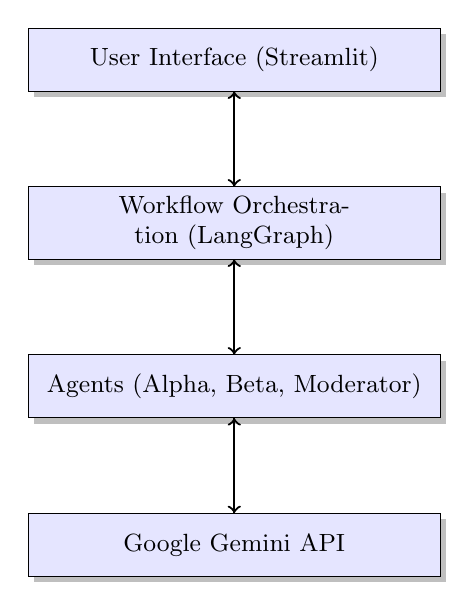
\begin{tikzpicture}[
    node distance=1.2cm,
    every node/.style={font=\small},
    box/.style={rectangle, draw, fill=blue!10, text width=5cm, text centered, minimum height=0.8cm, drop shadow},
    arrow/.style={->, thick}
]

% Layers
\node[box] (ui) {User Interface (Streamlit)};
\node[box, below=of ui] (workflow) {Workflow Orchestration (LangGraph)};
\node[box, below=of workflow] (agents) {Agents (Alpha, Beta, Moderator)};
\node[box, below=of agents] (api) {Google Gemini API};

% Arrows
\draw[arrow] (ui) -- (workflow);
\draw[arrow] (workflow) -- (agents);
\draw[arrow] (agents) -- (api);
\draw[arrow] (api) -- (agents);
\draw[arrow] (agents) -- (workflow);
\draw[arrow] (workflow) -- (ui);

\end{tikzpicture}
}
\caption{System Architecture showing the four-layer design}
\label{fig:architecture}
\end{figure}

\subsection{Agent Design and Characteristics}

We designed three specialized agents:

\subsubsection{Agent Alpha - Logical Debater}
Uses rational, evidence-based approach:
\begin{itemize}
\item Constructs arguments based on logical reasoning
\item Presents factual evidence and data
\item Maintains structured argument format
\item Adopts analytical tone
\end{itemize}

\subsubsection{Agent Beta - Emotional Debater}
Utilizes persuasive techniques:
\begin{itemize}
\item Emphasizes human impact and emotions
\item Employs rhetorical devices and narratives
\item Uses vivid, compelling language
\item Appeals to values and experiences
\end{itemize}

\subsubsection{Moderator Agent}
Serves as impartial judge:
\begin{itemize}
\item Reviews arguments objectively
\item Evaluates strength and coherence
\item Identifies logical errors
\item Declares winner with justification
\end{itemize}

\subsection{State Management}

The debate state tracks essential information:
\begin{itemize}
\item \textbf{Topic}: User-provided debate subject
\item \textbf{Positions}: Assigned stances for each agent
\item \textbf{Messages}: Complete argument history
\item \textbf{Round Counter}: Current round number
\item \textbf{Maximum Rounds}: Total rounds specified
\end{itemize}

This ensures agents have complete debate context when formulating responses.

\subsection{Debate Workflow}

The debate follows a structured process:
\begin{enumerate}
\item User submits topic and number of rounds
\item System detects position indicators ("vs", "versus")
\item Positions automatically assigned or self-determined
\item Agent Alpha presents opening (200 words)
\item Agent Beta responds (200 words)
\item System checks if maximum rounds reached
\item If not, return to Agent Alpha
\item If yes, Moderator judges (250-300 words)
\item Results displayed with full transcript
\end{enumerate}

\section{Implementation}

\subsection{Technology Stack}

Technologies used:
\begin{itemize}
\item \textbf{Python 3.13}: Primary language
\item \textbf{Streamlit 1.51}: Web interface
\item \textbf{LangGraph 1.0.3}: Multi-agent workflow orchestration
\item \textbf{Google Generative AI SDK 0.8.5}: Gemini API client
\item \textbf{Gemini 2.0 Flash}: Language model for content generation
\item \textbf{Pydantic}: Data validation
\end{itemize}

\subsection{Agent Configuration}

Agents configured with temperature 0.7 for balanced creativity and coherence. Maximum tokens set to 300 to maintain 200-word target. Each agent has specialized prompts defining personality and style. Agent Alpha emphasizes logic and evidence. Agent Beta encourages emotion and persuasion. Moderator focuses on objective evaluation.

\subsection{Automatic Position Assignment}

For topics with position indicators:
\begin{enumerate}
\item Convert topic to lowercase
\item Search for "vs" or "versus"
\item Split topic at separator
\item Assign first position to Alpha, second to Beta
\end{enumerate}

For other topics, agents determine opposing positions through their prompts.

\subsection{LangGraph Workflow}

Workflow implemented using StateGraph with three nodes (Agent Alpha, Agent Beta, Moderator). Entry point set to Agent Alpha. Alpha flows to Beta. Conditional edge from Beta checks rounds: if incomplete, return to Alpha; if complete, proceed to Moderator.

\subsection{Response Control}

Prompts explicitly instruct 200-word limit for agents and 250-300 words for Moderator. Token limit set to 300 as upper bound. This maintains balanced responses without post-processing.

\subsection{API Rate Limiting}

Added 2-second delay between API calls to comply with rate limits and prevent errors.

\subsection{User Interface}

Streamlit interface includes text input for topics, slider for rounds (1-5), start button, and real-time display. Messages color-coded: blue for Alpha, pink for Beta, orange for Moderator.

\section{Results and Evaluation}

\subsection{System Functionality}

We tested the system with various debate topics spanning different domains to evaluate its versatility and performance. Table I shows representative topics used during testing.

\begin{table}[htbp]
\caption{Sample Debate Topics Tested}
\begin{center}
\begin{tabular}{|l|c|}
\hline
\textbf{Topic} & \textbf{Rounds} \\
\hline
Cats vs Dogs & 3 \\
Remote Work vs Office Work & 3 \\
Electric Cars vs Gas Cars & 4 \\
Should AI replace teachers? & 3 \\
Climate change solutions & 4 \\
Universal basic income & 3 \\
Social media impact & 3 \\
\hline
\end{tabular}
\end{center}
\label{tab:topics}
\end{table}

\subsection{Debate Quality Assessment}

The system consistently generated coherent debates:
\begin{itemize}
\item Arguments relevant to topics
\item Agent Alpha used logical reasoning
\item Agent Beta used emotional appeals
\item Agents responded to each other's points
\item Moderator provided balanced evaluations
\item Response lengths stayed within limits
\end{itemize}

\subsection{Performance Metrics}

Response times measured:
\begin{itemize}
\item Agent response: 3-5 seconds
\item Moderator judgment: 5-7 seconds
\item 3-round debate: 45-60 seconds
\item 5-round debate: 70-90 seconds
\end{itemize}

Consistency achieved:
\begin{itemize}
\item 100\% position assignment success for "vs" topics
\item No position switching mid-debate
\item Consistent debate style adherence
\item Reliable round completion
\end{itemize}

\subsection{User Experience}

Informal testing with 5 users showed:
\begin{itemize}
\item Interface intuitive and easy to use
\item Debates engaging and relevant
\item Arguments well-reasoned
\item Winner decisions fair
\item Position assignment worked correctly
\item Color-coding helped distinguish agents
\end{itemize}

\section{Challenges and Solutions}

\subsection{API Rate Limiting}

\textbf{Challenge}: Rapid API calls caused rate limit errors.

\textbf{Solution}: Implemented 2-second delay between calls. This ensures compliance while keeping total debate time under one minute.

\subsection{Response Length Consistency}

\textbf{Challenge}: Inconsistent response lengths created imbalanced debates.

\textbf{Solution}: Added explicit word count instructions in prompts and set token limit to 300. This maintains balanced responses effectively.

\subsection{Position Assignment}

\textbf{Challenge}: For topics without "vs", agents sometimes argued similar positions.

\textbf{Solution}: Automatic detection for "vs" topics with position splitting. For others, prompts explicitly instruct agents to take opposing viewpoints.

\subsection{Fair Judgment}

\textbf{Challenge}: Early iterations showed moderator bias toward one agent.

\textbf{Solution}: Refined prompt with explicit criteria: argument strength, evidence use, logical consistency, and persuasiveness. Required specific examples from debate in judgment.

\subsection{Agent Differentiation}

\textbf{Challenge}: Agents initially sounded similar despite different styles.

\textbf{Solution}: Detailed prompts defining each style. Alpha uses formal language and analytics. Beta uses storytelling and emotion. Iterative refinement created distinct personalities.

\section{Computational Thinking Application}

\subsection{Decomposition}

We divided the system into independent modules:
\begin{itemize}
\item Input validation and position parsing
\item Agent creation and configuration
\item Debate state management
\item Workflow orchestration
\item UI rendering
\end{itemize}

Each module operates independently for easier testing and maintenance.

\subsection{Pattern Recognition}

We identified key patterns:
\begin{itemize}
\item Turn-taking: Alpha → Beta → Check rounds → Repeat or Judge
\item Argument structure: Claim → Evidence → Reasoning
\item Response pattern: Acknowledge → Counter → Conclude
\end{itemize}

\subsection{Abstraction}

We focused on essential information:
\begin{itemize}
\item State contains only needed data: topic, positions, messages, rounds
\item UI shows only relevant information
\item Prompts include only necessary context
\end{itemize}

\subsection{Algorithm Design}

Created systematic procedures:
\begin{itemize}
\item Position assignment: Detect "vs" → Split → Assign
\item Round management: Counter → Compare → Continue or Judge
\item Flow control: Alpha → Beta → Check → Route
\end{itemize}

\section{Future Work}

Potential enhancements:
\begin{itemize}
\item \textbf{Transcript Export}: Save debates as PDF or text files
\item \textbf{Multiple Agents}: Support panel discussions with 3+ agents
\item \textbf{Audio Integration}: Text-to-speech for listening to debates
\item \textbf{Human Participation}: Allow users to debate against AI
\item \textbf{Fact Verification}: Validate claims using external sources
\item \textbf{Audience Voting}: Let viewers vote for winners
\end{itemize}

Research directions:
\begin{itemize}
\item Study impact of agent personalities on debate quality
\item Compare AI debates with human debates
\item Develop improved judging methods
\item Explore educational applications
\end{itemize}

\section{Conclusion}

We developed a dual-agent debate system using Google Gemini API and LangGraph. The system features two agents with distinct styles: Agent Alpha uses logical reasoning while Agent Beta uses emotional appeals. A Moderator provides fair judgment.

Key features include automatic position assignment for "vs" topics, multi-round debate management with 200-word limits, and a Streamlit web interface. We applied computational thinking principles throughout: decomposition for modular design, pattern recognition for debate structure, abstraction for essential data, and algorithm design for systematic processes.

Testing showed the system generates coherent debates across diverse topics with distinct agent personalities. Response times average 3-5 seconds per agent. User feedback was positive regarding usability and debate quality.

Main challenges included API rate limiting (solved with 2-second delays), response length consistency (solved with prompt instructions), and agent differentiation (solved with detailed prompts).

This work demonstrates practical application of computational thinking in AI development and provides a foundation for future enhancements like transcript export, multiple agents, and human participation.

\section*{Acknowledgment}

We thank Dr. Shristi Sharma for her guidance on this project and Ahmedabad University for providing the necessary resources.

\begin{thebibliography}{00}

\bibitem{wooldridge1995}
M. Wooldridge and N. R. Jennings, ``Intelligent agents: Theory and practice,'' \textit{The Knowledge Engineering Review}, vol. 10, no. 2, pp. 115-152, 1995.

\bibitem{wing2006}
J. M. Wing, ``Computational thinking,'' \textit{Communications of the ACM}, vol. 49, no. 3, pp. 33-35, 2006.

\bibitem{vaswani2017}
A. Vaswani et al., ``Attention is all you need,'' in \textit{Advances in Neural Information Processing Systems}, vol. 30, 2017.

\bibitem{brown2020}
T. Brown et al., ``Language models are few-shot learners,'' in \textit{Advances in Neural Information Processing Systems}, vol. 33, pp. 1877-1901, 2020.

\bibitem{russell2020}
S. Russell and P. Norvig, \textit{Artificial Intelligence: A Modern Approach}, 4th ed. Pearson, 2020.

\bibitem{langgraph2024}
LangChain, ``LangGraph: Build stateful multi-agent applications,'' 2024. [Online]. Available: https://langchain-ai.github.io/langgraph/

\bibitem{gemini2024}
Google AI, ``Gemini API Documentation,'' 2024. [Online]. Available: https://ai.google.dev/docs

\bibitem{streamlit2024}
Streamlit Inc., ``Streamlit Documentation,'' 2024. [Online]. Available: https://docs.streamlit.io/

\end{thebibliography}

\end{document}
